\section{问题一：预热阶段的温度与含水率分布}

\subsection{问题分析}

问题一要求确定前 $1800\,\mathrm{s}$ 内药材的径向温度与含水率分布，并给出规定时空位置的结果。烘房环境随时间变化，药材内部响应滞后于表面，且水分扩散系数随含水率改变，因此需要建立时变边界下的非稳态传递模型。

根据模型准备中的基础方程，以附件 1 的环境数据和附录 2 的物性参数确定本问的初边值问题；采用径向离散和 BDF 自适应积分求解，通过收敛与守恒检验后，比较表面和内部的变化规律。

\subsection{模型建立}

\noindent\textbf{（1）径向近似}

题目给定药材长度 $L=0.25\,\mathrm{m}$、半径 $R_0=0.02\,\mathrm{m}$，初始温度为 $28\,{}^\circ\mathrm{C}$，初始干基含水率为 $2.55\,\mathrm{kg/kg}$。在共用假设基础上，本问采用以下局部简化：

\begin{enumerate}
  \item 预热阶段几何尺寸保持不变，热物性采用附录 2 给定的常数。
  \item 以远离端面的主体截面为研究对象，忽略该区域的轴向变化，仅考虑径向传递。
  \item 题目在问题 1 中未给出汽化潜热及相关相变参数，因此基础模型按照题面所给热物性参数建立，暂不显式考虑蒸发潜热反馈。
\end{enumerate}

由题目参数得到热扩散率 $\alpha=\frac{k}{\rho c_p}\approx1.689\times10^{-7}\,\mathrm{m^2/s}$。在 $1800\,\mathrm{s}$ 内，热扩散特征长度 $\sqrt{\alpha t}$ 约为 $1.74\,\mathrm{cm}$，远小于圆柱中央截面距端面的距离 $12.5\,\mathrm{cm}$；由 $D(C)\leq7\times10^{-9}\,\mathrm{m^2/s}$，水分扩散特征长度不超过 $0.36\,\mathrm{cm}$。结合均匀的侧壁环境，可将远离端面的主体截面近似为一维径向传递区域。

由附录 2，物性与对流参数取为
\[
\left\{
\begin{aligned}
\rho&=820\,\mathrm{kg/m^3},
&c_p&=2600\,\mathrm{J/(kg\cdot K)},\\
k&=0.36\,\mathrm{W/(m\cdot K)},
&h&=25\,\mathrm{W/(m^2\cdot K)},\\
h_m&=8\times10^{-7}\,\mathrm{m/s}.
\end{aligned}
\right.
\]

附件 1 在本问时间范围内提供每隔 $60\,\mathrm{s}$ 的环境数据。以分段线性插值构造 $T_\infty(t)$ 和 $C_\infty(t)$，保留原始采样值，不作时间外推。在本问条件下，\textbf{热传导和水分散失分别求解}。

\Needspace{13\baselineskip}
\noindent\textbf{（2）药材热传导}

将常热物性代入式~\eqref{eq:prep-heat}，结合均匀初温、圆心对称及表面对流换热条件，得到
\begin{equation}
\left\{
\begin{aligned}
\frac{\partial T}{\partial t}
&=\frac{\alpha}{r}\frac{\partial}{\partial r}
  \left(r\frac{\partial T}{\partial r}\right),\\
T(r,0)&=28,\\
\left.\frac{\partial T}{\partial r}\right|_{r=0}&=0,\\
-k\left.\frac{\partial T}{\partial r}\right|_{r=R_0}
&=h\left[T(R_0,t)-T_\infty(t)\right].
\end{aligned}
\right.
\label{eq:q1-heat-model}
\end{equation}
其中 $\alpha=\frac{k}{\rho c_p}$，温度以摄氏度表示。

\Needspace{16\baselineskip}
\noindent\textbf{（3）水分蒸发}

药材失水由\textbf{内部扩散和表面传质}共同决定。将附录 2 给出的有效扩散系数代入式~\eqref{eq:prep-moisture}，结合初始含水率和传质条件，得到
\begin{equation}
\left\{
\begin{aligned}
\frac{\partial C}{\partial t}
&=\frac{1}{r}\frac{\partial}{\partial r}
  \left(rD(C)\frac{\partial C}{\partial r}\right),\\
D(C)&=7\times10^{-9}\exp\left(-\frac{0.89}{C}\right),\\
C(r,0)&=2.55,\\
\left.\frac{\partial C}{\partial r}\right|_{r=0}&=0,\\
-D(C_s)\left.\frac{\partial C}{\partial r}\right|_{r=R_0}
&=h_m\left[C(R_0,t)-C_\infty(t)\right].
\end{aligned}
\right.
\label{eq:q1-moisture-model}
\end{equation}
其中 $C_s=C(R_0,t)$，含水率以 $\mathrm{kg/kg}$ 表示，扩散系数以 $\mathrm{m^2/s}$ 表示。两个控制方程均适用于 $0<r<R_0$、$0<t\leq1800\,\mathrm{s}$；本问不显式考虑蒸发潜热对温度场的反馈。

\input{sections/q1_numerics_text}

\Needspace{0.42\textheight}
\subsection{结果分析}

\Needspace{4\baselineskip}
\noindent\textbf{（1）温度分布}

规定时刻和径向位置的温度见表~\ref{tab:q1-temperature}，结果保留四位小数。

\input{tables/q1_temperature}

由表~\ref{tab:q1-temperature} 可知，\textbf{药材表面先升温，中心响应滞后}，这是由于表面直接与热风换热，而中心升温依赖内部导热。$1800\,\mathrm{s}$ 时，中心与表面温度相差 $3.2102\,{}^\circ\mathrm{C}$，且均低于同期烘房温度 $41.5130\,{}^\circ\mathrm{C}$，说明预热阶段结束时仍存在内外温差。

\Needspace{4\baselineskip}
\noindent\textbf{（2）含水率分布}

相同时空位置的干基含水率见表~\ref{tab:q1-moisture}。

\input{tables/q1_moisture}

由表~\ref{tab:q1-moisture} 可知，\textbf{失水主要集中在外层}。$1800\,\mathrm{s}$ 时，表面含水率已降至 $1.5102\,\mathrm{kg/kg}$，半径 $1\,\mathrm{cm}$ 处仍接近初值。中心结果在四位小数下为 $2.5500$，表明其变化很小。

\Needspace{0.62\textheight}
\noindent\textbf{（3）传递特征}

将温度和含水率的径向分布及时间变化绘于图~\ref{fig:q1-fields}。

\begin{figure}[H]
\centering
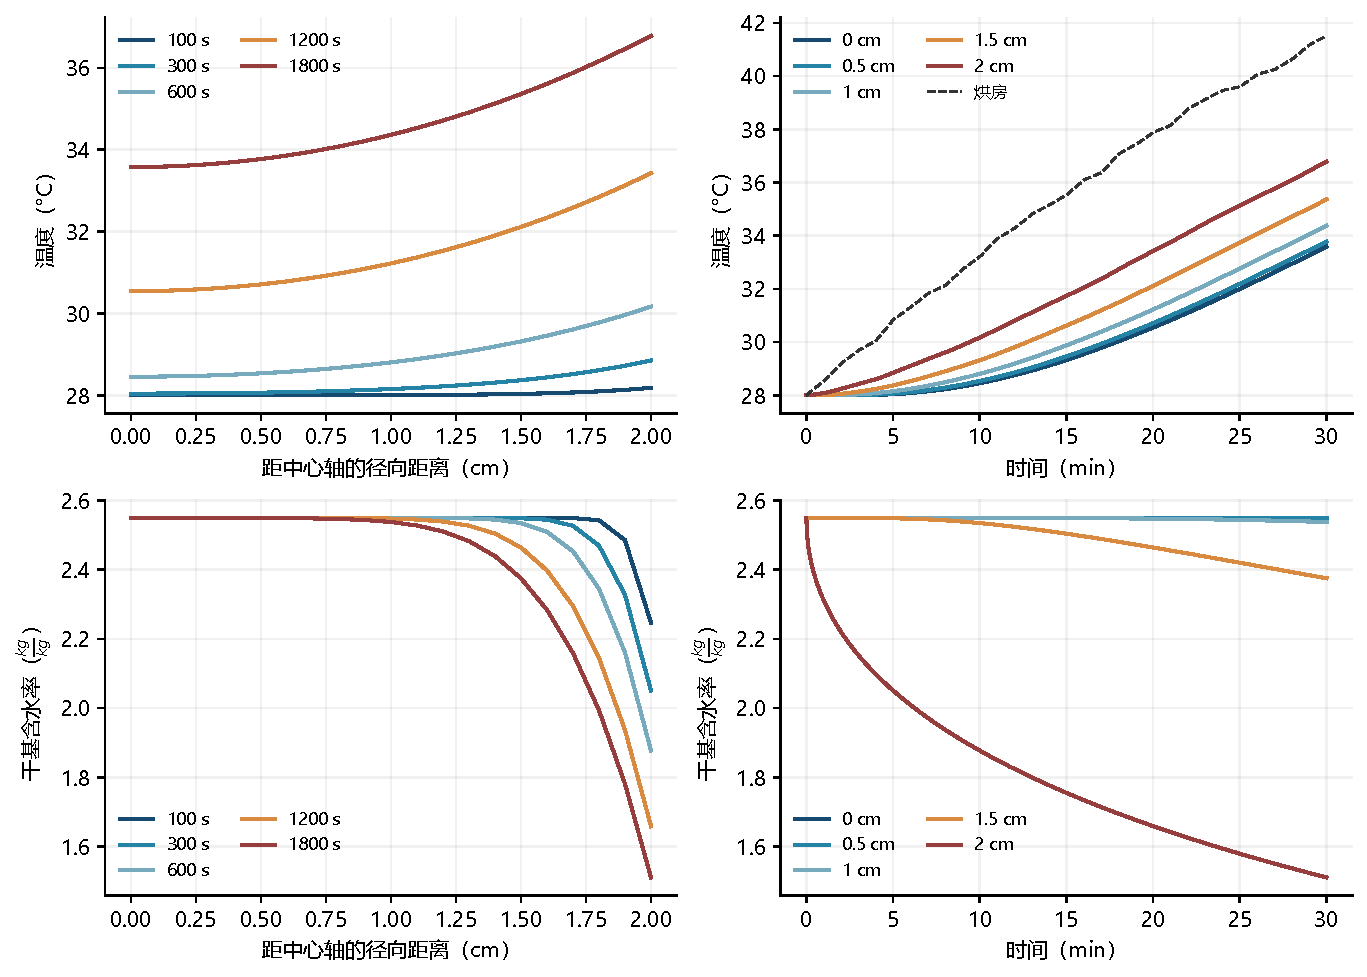
\includegraphics[width=\textwidth]{figures/q1_fields.pdf}
\caption{预热阶段温度与含水率的径向分布及时间变化}
\label{fig:q1-fields}
\end{figure}

图~\ref{fig:q1-fields} 显示，温度变化逐步传至中心，而明显失水仍局限于外层，与热扩散率高于水分扩散系数的量级关系一致。此外，$C$ 减小时 $D(C)$ 随之减小，外层干燥后水分向表面的扩散补给进一步受限。$1800\,\mathrm{s}$ 时，体积加权平均含水率由 $2.5500$ 降至 $2.2936\,\mathrm{kg/kg}$，下降 $10.0566\%$；结合径向差异可知，\textbf{此时药材尚未均匀干燥}。

本问得到的温度与含水率分布回答了预热阶段的时空变化问题。后续在此方程与数值处理框架中引入状态相关物性，可进一步描述全过程的传热传质。

